%
% File: chap02.tex
% Author: Oliver J. H. Feighan
% Description: delta-scf benchmarking, including dft and dftb methods.
% Talk about important factors for modelling LHII
%
%\let\textcircled=\pgftextcircled
\chapter{Mean-Field excited states}
\label{chap:dscf}

\subsubsection*{Previous Published Work}
The work presented in this chapter is based on joint work with Dr Susannah Bourne-Worster,
and was published in March 2021\cite{Worster2021}. The account given in this 
chapter includes research that was also reported in this publication, namely the
parts of section \ref{sec:benchmarking} from \ref{subsec:reference_data} up to
but excluding \ref{subsec:dscf_gfn_tests}.

\initial {T}his chapter collates all of the work done on investigating and benchmarking
\dscf methods, at both an ab initio DFT level of theory as well as with semi-empirical, 
tight-binding approximations. The reduced cost and moderate accuracy of these methods
make them an ideal substitute for full TD-DFT or high-level methods when investigating
large systems like chlorophyll.
Transition properties were calculated for a range of molecules, as well as
for a small set of chlorophyll geometries, using variety of different basis sets,
density functionals, response methods and electronic structure methods. Most of 
the work was compared to either high-standard EOM-CCSD or SCS-CC2 reference, from
which conclusions were made on the accuracy of each method. The non-orthogonality 
issue of the ground and excited states were also investigatede for the mean-field 
\dscf method, as well as assignment of transitions based on symmetry. 
It was found that while the DFT methods give reasonable results, the semi-empirical
\dscf methods are not as accurate. This result is unexpected in the context of
the benchmarking, however has reasonable explanations, and will guide the work
of the later chapter on developing a new semi-empirical method.

%=======
\section{Theory}
\label{sec:dscf_theory}
\subsection{$\Delta$-SCF and eigenvalue difference}
\label{subsec{dscf_and_eigdiff}}

\dscf predicts the transition energy $\Delta E$ of a system as the difference of
the single point energy $E_n$ of two states:

\begin{equation}
\Delta E = E_{2} - E_{1}
\end{equation}

Finding the excited state correctly can be an issue, and for ease is usually assumed
to be similar to the ground state. In its simplest form, the \dscf method calculates
the ground state with normal DFT or other mean-field methods, and
then calculates the excited state by rerunning the same method with the excited
state occupation numbers. A full description of both the ground as excited state
is given as the orbital coefficients output from the two calculations.

Initially, the excited state was calculated by relaxing the orbitals which
contain the excited electron and hole in the ground state space, so that the
excited state and ground state are orthogonal\cite{Hunt1969}. However, it was
argued that this procedure would exacerbate errors from finding the ground
state, and that the excited state was not a proper SCF solution\cite{Gilbert2008}.
Alternatively, an SCF like method was proposed, where instead of
populating orbitals according to the aufbau principle, orbitals which most
resemble the previous iteration's orbitals should be occupied. Each iteration 
in an SCF procedure produces new molecular orbital coefficients by solving the 
Roothaan-Hall equations\cite{Roothaan1951}, generally given as an eigenvalue problem:

\begin{equation}
\mathbf{F} \mathbf{C}^{\text{new}} = \mathbf{S} \mathbf{C}^{\text{new}} \epsilon
\end{equation}

where $\mathbf{C}^{\text{new}}$ are the next orbital coefficient solutions, 
$\mathbf{S}$ is the overlap, and $\epsilon$ are the orbital energies. 
The Fock matrix $\mathbf{F}$ is calculated from the previous set of orbital 
coefficients:

\begin{equation}
\mathbf{F} = f\left(\mathbf{C}^{\text{old}}\right)
\end{equation}

The amount of similarity of orbitals can be estimated from their overlap:

\begin{equation}
\mathbf{O} = \left(\mathbf{C}^{\text{old}}\right)^\dagger \mathbf{S} \mathbf{C}^{\text{new}}
\end{equation}

and for a single orbital can be evaluated as a projection:

\begin{equation}
p_j = \sum^n_i O_{ij} = \sum^N_\nu \left[\sum^N_\mu\left(\sum^n_i C_{i\mu}^{\text{old}}\right)S_{\mu\nu}\right]C^{\text{new}}_{\nu j}
\end{equation}

where $\mu,\nu$ are orbital indices. The population can then be given by the set
of orbitals with the highest projection $p_j$.  This method can be used for any
excited state, with the caveat that the orbital solution will most likely be in
the same region as the ground state solution. For a small number of low lying states,
this is generally  true, and so \dscf can be used to calculate a small spectrum of
excited states\cite{Gilbert2008}. The method of using this orbital overlap is called
the maximum overlap method (MOM)\cite{Gilbert2008}.

\dscf has been shown to be cheap alternative to TD-DFT and other higher level
methods\cite{Liu2004, Gavnholt2008, Besley2009}, without considerable losses of
accuracy in certain cases, especially for HOMO-LUMO transitions\cite{Kowalczyk2011}.
Additionally, as the excited state is given as solutions to SCF equations,
the gradient of this solution can be given by normal mean-field theory.
These gradients would be much cheaper than TD-DFT or coupled cluster methods, and
so would be better for any dynamic simulation\cite{Gavnholt2008}.

\subsection{Eigenvalue Difference}
\label{subsec:eigval_diff}
Another approximation to full response theory would be to eigenvalue difference method. 
Here there is assumed to be no response of the orbital energies and shapes when 
interacting with light. This would be recovered from the complete Cassida equation
if the coupling elements in the $\mathbf{A}$ and $\mathbf{B}$ matrices are set to zero.
This gives the difference between the excited state energy and the ground state
energy, the transition energy, as just the difference of the orbital energies between
the orbital an electron has been excited ($\epsilon_{\text{e}}$) to and the orbital
has been excited from ($\epsilon_{\text{g}}$):

\begin{equation}
\Delta E = \epsilon_{\text{e}} - \epsilon_{\text{g}}
\end{equation}

Additionally, transition properties can be calculated by construction transition 
density matrices from only the ground state solution, needing only a single SCF optimization. 
Generally, eigenvalue difference methods are not seen as accurate response methods,
but can offer a quick and easy initial value\cite{Gimon2009}.

\subsection{Transition Density and Dipole Moments}
\label{subsec:dscf_transition_density}
\dscf transition properties, such as the transition dipole moment, can be calculated from
the SCF solutions for the ground and excited states. The reduced one-particle transition
density matrix $\mathbf{D}^{21}$ can be written as:

\begin{equation}
\mathbf{D}^{21} = \ket{\Psi_1} \bra{\Psi_2}
\end{equation}

where $\ket{\Psi_n}$ is the Slater determinant of state $n$, constructed from the
set of spin orbitals $\{ \phi_{j}^{\left(n\right)} \} $. Expressed 
in terms of the molecular orbitals coefficients $\mathbf{C}^{\left(n\right)}$, the
transition density matrix is given by

\begin{equation}
\mathbf{D}^{21} = \mathbf{C}^{\left(2\right)} \text{adj}\left(\mathbf{S}^{21}\right) \mathbf{C}^{\left(1\right) \dagger}
\end{equation}

where $\mathbf{S}^{mn}$ is the overlap of the two states. The adjunct of the overlap
correspond to L{\"o}wdin's normal rules for non-orthogonal determinants \cite{Lowdin1955}.
For transition dipole elements, this is:

\begin{equation}
\braket{\Psi_2|\hat{\mathbf{\mu}}|\Psi_1} = \sum_{jk} \mathbf{\mu}_{jk}^{21} \text{adj} \left( \mathbf{S}^{21}\right)_{jk}
\end{equation}

where $\hat{\mathbf{\mu}}$ is the one-electron transition dipole operator, and
$\mu_{jk}$ is the element of this operator corresponding to orbital indices $j$, $k$.
The determinant of this overlap, the orbital inner products, can be defined as the
inner product of the two states:

\begin{equation}
\left\lvert {\mathbf{S}^{21}} \right\rvert = \braket{\Psi_2|\Psi_1}
\end{equation}

The general definition of the transition dipole

\begin{equation}
\mathbf{\mu}^{1\rightarrow2} = \braket{\Psi_2|\hat{\mathbf{\mu}}|\Psi_1}
\end{equation}

can be expressed with this transition density matrix as:

\begin{equation}
\begin{split}    
\braket{\Psi_2|\hat{\mathbf{\mu}}|\Psi_1} &= \text{tr}\left(\hat{\mathbf{\mu}} \ket{\Psi_1} \bra{\Psi_2} \right) \\
&= \text{tr}\left( \hat{\mathbf{\mu}} \mathbf{D}^{21}\right)
\end{split}
\end{equation}

\subsection{Semi-empirical extensions}
\label{subsec:dscf_xtb}
A main investigation of this chapter is whether the range of DFT methods
that could be used for \dscf and eigenvalue difference methods could be extended 
by using tight-binding methods to predict transition properties.
This mainly focused on the recently published GFN-xTB method, parameterized by
the Grimme group \cite{Grimme2017}. This method has been parameterized for geometries,
frequencies and non-covalent interactions, and uses an extended version of H{\"u}ckel theory.
The name GFN-xTB is acronym for "Geometries, Frequencies, Non-Covalent - eXtended Tight Binding".
This method was chosen for two reasons. The first being that the GFN-xTB method was
already implemented in the \code{QCORE} package. This significantly reduced the
amount of effort required for this project. Additionally, there would be other
users and developers who would help with implementation of this new method.
Second is that a similar method has already been published that calculates
transition properties, the precursor to the GFN-xTB methods. This is the sTDA-xTB
method \cite{Grimme2016}.

\subsubsection{sTDA-xTB}
\label{subsubsec:stda_xtb}
sTDA-xTB ("simplified Tann-Dancoff Approximation - eXtended Tight Binding") is another
method in the family of xTB methods developed by the Grimme group, and is parameterised
for transition properties. The accuracy in calculating transition energies with this
method is very good, with the error to high-level results being around 0.3 - 0.5 eV.

Similar to other xTB methods, the sTDA-xTB method is a tight-binding method that
uses empirically fit parameters and a minimal basis set. It was trained on a
test set of highly accurate coupled cluster and density functional theory
excitation energies, as well as atomic partial charges for inter-electronic interactions.

Unlike other xTB methods, coefficients in the basis set for sTDA-xTB are dependent on the D3
coordination number. This makes basis functions far more flexible, which would usually
be achieved in with fixed basis functions by using diffuse or other additional orbitals in
the basis set. Additionally, it uses two sets of parameterized basis sets - a
smaller valence basis set (VBS) and an extended basis set (XBS). Whilst this reduces
the cost of having larger basis sets, it makes calculating the gradient of transition
properties much more difficult. 

The two basis sets are used to construct formally similar Fock matrix elements,
however in practice they use different global parameters. The core Hamiltonian
is similar to other DFTB methods that use a self-consistent charge (SCC) method, as
opposed to an SCF method, to obtain molecular orbital coefficients. It is given by:

\begin{equation}
\bra{\psi_\mu} H^{\text{EHT, sTDA-xTB}} \ket{\psi_\mu}= \frac{1}{2} \left(k^l_\mu k^{l'}_\nu\right) \frac{1}{2} \left(h^l_\mu h^{l'}_\nu\right) S_{\mu\nu} - k_T \bra{\psi_\mu}\hat{T}\ket{\psi_\nu}
\end{equation}

where, $\mu,\nu,l,l'$ are orbital and shell indices  $k^l_\mu$ are shell-wise 
H{\"u}ckel parameters, $h$ are effective atomic-orbital energy levels, $S$ is
the overlap, $k_T$ is a global constant and $\hat{T}$ is the kinetic energy 
operator. The charges used in the inter-electronic repulsion function are given 
by CM5 \cite{Marenich2012} charges for the XBS Fock matrix. These are calculated
using Mulliken charges obtained from diagonalising the Fock matrix with the VBS. 
The charges for the initial VBS Fock matrix are based on Gasteiger charges \cite{Gasteiger1978},
modified by the parameterised electronegativities of atoms in the system.

The whole process for determining molecular orbitals can be summarized as:
\begin{enumerate}
	\item Calculate modified Gasteiger charges for the first initial guess
	\item Diagonalise Fock matrix in the VBS to get the first set of Mulliken charges
	\item Compute CM5 charges
	\item Diagonalise Fock matrix in the VBS again for final set of Mulliken charges.
	\item Recalculate CM5 charges with this final set, and diagonalize the Fock matrix in the XBS. The molecular orbital coefficients from this are then fed to the response theory.
\end{enumerate}

The response theory for this method is based on the previous work in the Grimme 
group on the simplified Tamm-Dancoff Approximation \cite{Grimme2013}.
There are several approximations made between full linear response theory and
the sTDA method. First is the Tamm-Danncoff approximation, where the $\mathbf{B}$
matrix is ignored. The second approximation is to use monopole approximations with
Mataga-Nishimoto-Ohno-Klopman operators instead of explicit 2 electron integrals
to calculate matrix elements, as well as neglecting the density functional term.

Transition charges are used to calculate these MNOK integrals. The charge $q^A_{nm}$,
the charge centred on atom $A$ given by transition density for the transition of
$ n \rightarrow m$, are computed using a Löwdin population analysis:

\begin{equation}
q_{nm}^A = \sum_{\mu \in A} C^`_{\mu n} C^`_{\mu m}
\end{equation}

where the transformed coefficients $C^`_{\mu n}$ are given by the orthogonalising
the original MO coefficients $\textbf{C}$:

\begin{equation}
\textbf{C}^` = \textbf{S}^{\frac{1}{2}} \textbf{C}
\end{equation}

and $\mu$ is an index that runs over the atomic orbitals (AO).

The operator is the 
MNOK\cite{Nishimoto1957}\cite{Ohno1964}\cite{Klopman1964} damped coloub function, 
with different exponents $y_K$ and $y_J$ for exchange and coulomb integral respectively. 
The $a_x$ parameter is included to recover the amount of Fock exchange mixing in
the original matrix element equation, and is a free parameter. These will be discussed
in more detail in the next chapter, as they are a crucial part of designing a new
response method for chlorophyll systems.

Third is the truncation of single particle excited space that is used to construct 
the $\mathbf{A}$ matrix. This reduces the number of elements that need to be 
calculated, and so reduces the time taken for diagonalisation, whilst also capturing 
a broad enough spectrum of excitation energies. The sTDA-xTB has many of the same 
goals as this project, except in one respect, which is the gradient theory. As 
the sTDA-xTB method still requires constructing and diagonalizing the $\mathbf{A}$ 
matrix, albeit with a tight-binding method for molecular orbital coefficients, 
the gradient of the transition properties would still be difficult to calculate.

\section{Benchmarking}
\label{sec:benchmarking}
The first step in testing whether a GFN-xTB based \dscf method (which we
name \dxtb) could predict TD-DFT transition properties with decent accuracy was
to test a set of small molecules, as well as bacterial chlorophylls
from the LHII protein against high-level results.

\subsection{Reference Data and test set}
\label{subsec:reference_data}
The test set comprised of 109 small molecules. Each system was closed-shell, 
contained 12 atoms or less, and contained on H, C, N, O and F atoms. The size and
relative simplicity of this test set was chosen to minimise any other factors that
could cause complication in analysing the results. For example choosing a consistently
correct basis set and functional for the \dscf results would have been challening 
if it was necessary to include transition metal complexes, as well considering
CPU walltime contraints. Additionally, the size of these molecules made symmetries
much easier to inspect by hand.

Reference data was calculated as the three lowest energy singlet excited states, 
using EOM-CCSD with an aug-cc-pVTZ basis set. These results were generated
using the Gaussian 16 program \cite{Gaussian16}.

\subsection{Small Systems}
\label{subsec:smalltest}
Transition properties for this test set were calculated using TD-DFT and \dscf,
both using a CAM-B3LYP functional and aug-cc-pVTZ basis set. The transitions were
assigned to the EOM-CCSD results by comparing transition dipoles, energies and 
the character of the MOs involved in the transitions. Where the symmetries could
be assigned, these were also used, however this was not the case for all systems
as many were unsuccessful in labelling symmetry or defaulted to a non-Abelain group.
Symmetry labelling was also only available for TD-DFT calculations, as these were
performed with Gaussian 16. \dscf calculations were done with the \code{QCORE}
program.

The \dscf singlet transition is not a correct representation of a 
true singlet excitation, as this is a superposition of both spin-same
 $\alpha \rightarrow a, \alpha$ and spin-flipping $\alpha \rightarrow a, \beta$
excitations. The spin-purification formula:

\begin{equation}
\Delta E_S = 2\Delta E^{i,\alpha \rightarrow a, \alpha} - \Delta E^{i,\alpha \rightarrow a, \beta}
\end{equation}

was used to correct for the true singlet excitation energy $\Delta E_S$.

The results of comparing transition energies and transition dipole magnitudes are
shown in figures \ref{fig:energy_scatter} and \ref{fig:dipole_scatter}.

\begin{figure}
\centering
\includegraphics[scale=0.6]{../../Year_3/dscf_figures/energy_scatter.png}
\caption{Transition energies $\Delta E$ from TD-DFT (black) and \dscf (red)
 plotted against EOM-CCSD energies, with the line $y=x$ (dashed) for reference.
 The ethene dimer outlier has been circled.}
\label{fig:energy_scatter}
\end{figure}

\begin{figure}
\centering
\includegraphics[scale=0.6]{../../Year_3/dscf_figures/dipole_scatter.png}
\caption{Transition dipole magnitudes from TD-DFT (black) and \dscf (red) plotted
against EOM-CCSD transition dipole magnitudes, with the line $y=x$ (dashed) for 
reference.}
\label{fig:dipole_scatter}
\end{figure}

Overall, the excitation energies calculated with \dscf are as accurate at predicting
EOM-CCSD energies as TD-DFT. The mean error is 0.35 eV, with a standard deviation
of 0.25 eV. This is a marginal improvement on the TD-DFT results, which has a mean
and standard deviation of 0.41 eV and 0.27 eV respectively. Transition dipoles 
were similarly accurate to the reference data, although \dscf performs slightly 
worse in this respect. The mean and standard deviation in the absolute value
of transition dipole moment, $|\mathbf{\mu}|$, was 0.07 a.u. and 0.08 a.u. respectively.
For TD-DFT, the mean and standard deviation were 0.03 a.u. and 0.06 a.u. (the atomic
unit here being equal to $ea_0$).
The outlier circled in figure \ref{fig:energy_scatter} is an ethene dimer system,
and shows the inability of \dscf to capture a mixed excited state. The two LUMO
orbitals in this dimer system are in-phase and out-of-phase combinations of the 
$\pi$-antibonding orbitals, which are very close in energy. The HOMO
orbitals are the same on both ethene molecules, being the $\pi$-bonding orbitals, 
which are degenerate in energy. The first excited state is predicted by TD-DFT and
EOM-CCSD to be a mix of these two close HOMO-LUMO transitions, however \dscf cannot
include this mixed behaviour. \dscf predicts two transitions of 7 eV and 10 eV,
whilst TD-DFT and EOM-CCSD predict 7.5 eV.

In summary, \dscf can be seen to accurately predict transition properties
to a EOM-CCSD level of accuracy with as much success as TD-DFT, except in cases
of mixed transitions. It might then be expected a tight-binding method, with good electronic 
structure treatment, could also be accurate whilst drastically reducing
the cost of calculation. 

\subsection{Non-orthogonality}
\label{subsec:dscf_nonorth}
There is, however, another caveat with \dscf. The ground and excited states, solutions
to two separate SCF cycles, will not be truly orthogonal. The
Slater determinants $\ket{\Psi_n}$, are constructed from the set of orbitals 
$\{ \ket{\phi_j^{\left(n\right)}} \}$ that will be orthogonal within the same state,
however the overall states will not be orthogonal to each other, such that the inner product:

\begin{equation}
S^{21}_{jk} = \braket{\phi_j^{\left(2\right)} | \phi_k^{\left(1\right)}}
\end{equation}

will be non-zero. Similarly, there will be a non-zero transition charge:

\begin{equation}
q^{21} = \braket{\Psi^2|\Psi^2}
\end{equation}

which breaks the origin-independence property of the transition dipole moment. In
this way, any transition dipoles that do not have their centre at the origin will
have a systematic error based on this overlap and the distance from the origin.
For vertical transitions, this transition charge should be zero, and so all transition
dipole moments calculated with non-orthogonal \dscf would always have this error.

In order to fix this issue, a transformation to symmetrically orthogonalise the two states
was applied, which also would preserve as much character of the original states as possible.
The transformation is given by:

\begin{equation}
\ket{\Psi_{\tilde{\nu}}} = \sum_{\nu} \ket{\Psi_\nu} \left[\mathbf{S}^{-\frac{1}{2}} \right]_{\nu\tilde{\nu}}
\end{equation}

where $\mathbf{S}$ here is a block matrix:

\begin{equation}
\mathbf{S} = \begin{pmatrix}
    1 & S \\
    S & 1 
\end{pmatrix}
\end{equation}

with $S$ being the overlap value of the two states $\braket{\Psi_2|\Psi_1}$.

\begin{figure}
\centering
\includegraphics[scale=0.6]{../../Year_3/dscf_figures/correction_scatter.png}
\label{fig:correction_scatter}
\caption{The absolute value of the error in transition dipole magnitude between
\dscf and EOM-CCSD, plotted against the \dscf overlap of the ground and excited
state. All systems were translated by 100 \AA   in all cartesian axes. Transition
dipole magnitudes calculated without any correction are shown in red, whilst
those with the symmetric orthogonalisation correction are shown in black.}
\end{figure}

It was found that using this method for correcting the non-zero overlap of states, 
the origin-independence of the transition dipole moment was recovered (see figure
\ref{fig:correction_scatter}).
The transition dipole for each molecule in the test set systems was calculated
for molecules translated by 100\AA  in each of the $x$, $y$ and $z$ axes.
This would induce an error for the non-orthogonalised states, which has been
corrected for in the calculations with the symmetric orothogonalistion.
It should be noted that whilst this effect is dependent on how large the overlap may be, and
it could be argued that with a small overlap this effect may not be large, having 
any large translation of the molecule (on the order of hundreds of angstroms) can
lead to nonphysical transition dipole magnitudes. In a large protein system, where
these distances can be on this scale, this would obviously present a much larger problem
than for a vacuum phase small molecule.

\subsection{LHII Chlorophyll}
\label{subsec:dscf_chl_tests}
The accuracy of \dscf was also tested on a set of bacterial chlorophyll A (BChla) 
molecules. These are a much larger and more complex system, and so present a tougher
challenge for the \dscf method. Additionally, it is a more relevant test for the
goal of simulating a whole LHII complex.

As each BChla is 140 atoms, EOM-CCSD could not be used as the reference method due
to resource constraints, so TD-DFT at a PBE0/Def2-SVP level of theory was used instead \cite{Adamo1999, Schafer1992}.
This has been used previously for BChla structures, and has been shown to be a good
balance between accuracy and cost \cite{Stross2016}. 
The \dscf was run with the same density functional and basis set.

\begin{figure}
\centering
\includegraphics[scale=0.6]{../../Year_3/dscf_figures/chlorophyll_energy_scatter.png}
\label{fig:chl_energy}
\caption{The transition energies from \dscf for the 26 chlorophyll geometries, 
plotted against energies from TD-DFT. The line of best fit ($R^2=0.87$) is shown 
as the dashed line.}
\end{figure}

\begin{figure}
\centering
\includegraphics[scale=0.6]{../../Year_3/dscf_figures/chlorophyll_dipole_scatter.png}
\caption{The transition dipole magnitudes from \dscf for the 26 chlorophyll geometries, 
plotted against dipole magnitudes from TD-DFT. The line of best fit ($R^2= 0.57$) 
is shown as the dashed line.}
\label{fig:chl_dipole}
\end{figure}

\dscf can be seen to give transition energies to within the accuracy of TD-DFT, 
such that the variations in transition energy can be said to be due to
physical intra-molecular reasons rather than random error from the \dscf method.
\dscf could therefore be used to accurately predict geometry dependent properties.

However, the error in transition dipole magnitudes is larger than that of the small
test set. This error is about 0.42 a.u. larger, but without EOM-CCSD or another
high-level method, it's unclear whether this error might be from TD-DFT or \dscf.
Additionally, there is a clear correlation between the transition dipole magnitudes
from TD-DFT and \dscf, and so whilst quantitative statements cannot be made, qualitative
assessments can be confidently made from \dscf data.

\afterpartskip
\subsection{xTB methods}
\label{subsec:dscf_gfn_tests}
The same benchmarking set was used with the \dxtb method. The number of methods
in the comparison was also expanded to cover a range of approximations in calculating
transition properties, including the aforementioned sTDA-xTB method. To include 
this in the comparison, it was necessary to use the spin-component-scaled second
order coupled-cluster (SCS-CC2) \cite{Hattig2000, Hellweg2008} reference data produced
by the Grimme group.
Concurrent to this work, the GFN0-xTB method was also implemented in \code{QCORE}.
This method is similar to the GFN1-xTB method, but excludes any charge dependent
terms in its Fock matrix so is not self-consistent. This method therefore only
uses a single diagonalisation, with orbital solutions being the same for both
ground and excited state. A transition energy from \dscf with this method would
functionally be the same as an eigenvalue difference, and this was included in 
the benchmarking to test whether it would be a possibility for predicting transition
properties.
Also included in this benchmarking is using the eigenvalue differences from
sTDA-xTB, given by the \code{xtb4stda} program, to observe how much improvement
to transition properties is caused by the sTDA procedure. \code{xtb4stda} is the 
first of two programs that runs a version of xTB, providing molecular orbital
coefficients and energies for the sTDA program to then use to calculate the transition
properties.

All methods included were:
\begin{itemize}
    \item High level TD-DFT, with a range separated functional CAM-B3LYP and
     a aug-cc-pVTZ basis set.
    \item Lower level TD-DFT, with a PBE0 functional and smaller Def2-SVP basis set.
    \item \dscf with CAM-B3LYP/aug-cc-pVTZ.
    \item \dscf with PBE0/Def2-SVP.
    \item linear response with GFN1-xTB and GFN0-xTB.
    \item \dscf with GFN1-xTB and GFN0-xTB, named \dxtb.
    \item Full sTDA-xTB, for additional reference.
    \item sTDA-xTB eigenvalue difference.
\end{itemize}

A source of error that hasn't been discussed in much detail so far is
the assignment of transitions between different methods. A known problem of \dscf
methods is that the excited state SCF cycle may not converge to the correct state,
or it might collapse back to the ground state. This could be seen in the symmetry
of the excitation, as if \dscf excited state has converged to different transition
than TD-DFT and CC2 it would have different symmetries of transition. The benchmarking discussed
above used symmetry labels to assign TD-DFT transitions to EOM-CCSD, but as noted
earlier this was not always possible, and assigning symmetry labels to \dscf was 
not possible. Instead, transition dipole orientations and plots of MOs were used
as a proxy. This proved harder in the \dxtb case for two reasons. First is the
valence basis set for the \dxtb calculations are very different to those used in
DFT. Second is that this information was not available for the CC2 data, however
the symmetry labels were. Additionally, inspecting the symmetry is very time-consuming
and can not be automated. Every new method that was added to the benchmarking
had to have every molecule individually inspected to make sure the symmetry
of each transition was correct. Assigning symmetry to \dscf results was investigated,
but was not a straightforward implementation.
 
\subsubsection{Post-SCF Assignment of Symmetry}
\label{subsubsec:post_scf_symmetry}

Considering symmetry is a common thread in many parts of electronic structure 
theory. It appears in normal mode analysis, wave-function analysis and assignment
of electronic transitions. For this project, assigning symmetry to the transitions
for \dscf would require assigning symmetry to the MOs and overall wave-function of
a molecule.
Broadly speaking, most electronic structure codes have two choices in assigning
symmetry to orbitals - either all of the SCF code will treat symmetry from the 
outset, or nothing is assigned in the SCF code and assignment will happen post-SCF.
Both these approaches have benefits and drawbacks. The first method allows the 
symmetry to be given at any point in the SCF procedure, and allows the Hamiltonian
to be organized into a block diagonal matrix. This can be useful when solving
for a large basis set or large system as the matrix diagonalisation can be
partitioned and parallelised over several cores or nodes on a cluster computer.
However, this works best if the system is highly symmetric, which is often not
the case when treating unoptimized systems, such as those from a molecular dynamics
simulation, and is definitely not the case when looking at biological systems.
The second approach, assigning symmetry after the SCF cycles, doesn't fix these
drawbacks, but it does allow for codes which originally didn't have symmetry
assignment to be extended without rewriting SCF code. The obvious drawback of
doing assignment post-SCF is that symmetry can't be utilized during the SCF procedure.
The second approach was opted for, as this was the easiest to implement in \code{QCORE}.
The open source library libmsym \cite{libmsym} was used for point group assignment
routines and finding the symmetry adapted linear combination of atomic orbitals.
The steps for assigning orbital symmetry is as follows:

\begin{enumerate}
    \item Determine the point group of the molecule, from the atomic positions
    \item Setup the atomic orbitals in the libmsym representation.
    \item Get the symmetry adapted linear combinations (SALCs) of atomic orbitals for 
    each subspace. These subspaces are the groups of symmetries that can be found
    in the point group of the molecule.
    \item The SALCs can then be used to construct the transformation matrix $T$.
    \item Assign the one electron molecular orbital (MO) for these subspace characters
     with the symmetry adapted linear combinations.
    \item Multiply the one electron MO symmetries together to find the symmetry 
    of the overall wavefunction.
\end{enumerate}

\begin{figure}
    \centering
    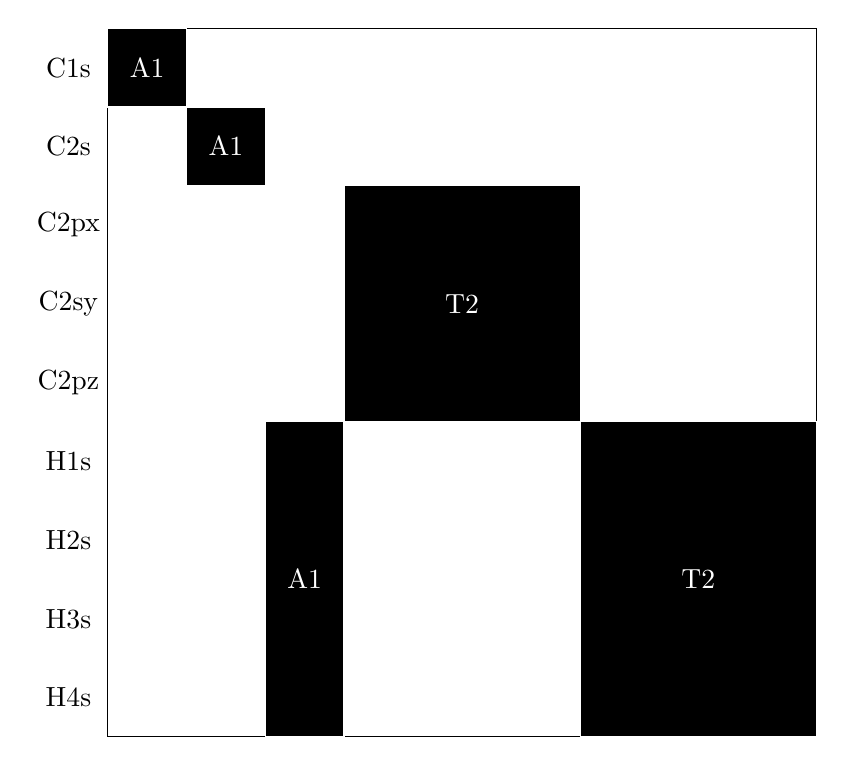
\begin{tikzpicture}
        \node[draw=none,
        rectangle, 
        minimum width = 1cm, 
        minimum height = 1cm
        ](r) at (-5cm,4cm) {C1s};
        \node[draw=none,
        rectangle, 
        minimum width = 1cm, 
        minimum height = 1cm
        ](r) at (-5cm,3cm) {C2s};
        \node[draw=none,
        rectangle, 
        minimum width = 1cm, 
        minimum height = 1cm
        ](r) at (-5cm,2cm) {C2px};
        \node[draw=none,
        rectangle, 
        minimum width = 1cm, 
        minimum height = 1cm
        ](r) at (-5cm,1cm) {C2sy};
        \node[draw=none,
        rectangle, 
        minimum width = 1cm, 
        minimum height = 1cm
        ](r) at (-5cm,0cm) {C2pz};
        \node[draw=none,
        rectangle, 
        minimum width = 1cm, 
        minimum height = 1cm
        ](r) at (-5cm,-1cm) {H1s};
        \node[draw=none,
        rectangle, 
        minimum width = 1cm, 
        minimum height = 1cm
        ](r) at (-5cm,-2cm) {H2s};
        \node[draw=none,
        rectangle, 
        minimum width = 1cm, 
        minimum height = 1cm
        ](r) at (-5cm,-3cm) {H3s};
        \node[draw=none,
        rectangle, 
        minimum width = 1cm, 
        minimum height = 1cm
        ](r) at (-5cm,-4cm) {H4s};
        
        \node[draw,
        rectangle, 
        minimum width = 9cm, 
        minimum height = 9cm
        ](r) at (0cm,0cm) {};

        \node[draw,
        rectangle, 
        color=white,
        fill=black,
        minimum width = 1cm, 
        minimum height = 1cm
        ](r) at (-4cm,4cm) {A1};

        \node[draw,
        rectangle,
        color=white, 
        fill=black,
        minimum width = 1cm, 
        minimum height = 1cm
        ](r) at (-3cm,3cm) {A1};

        \node[draw,
        rectangle,
        color=white,
        fill=black,
        minimum width = 1cm, 
        minimum height = 4cm
        ](r) at (-2cm,-2.5cm) {A1};

        \node[draw,
        rectangle, 
        color=white,
        fill=black,
        minimum width = 3cm, 
        minimum height = 3cm
        ](r) at (0cm,1cm) {T2};

        \node[draw,
        rectangle, 
        color=white,
        fill=black,
        minimum width = 3cm, 
        minimum height = 4cm
        ](r) at (3cm,-2.5cm) {T2};

    \end{tikzpicture}
    \caption{A breakdown of the symmetry orbitals in STO-3G methane into the subspaces 
    present in the T\textsubscript{d} point group.}
\end{figure}

This procedure was implemented and tested on methane with a minimal STO-3G basis set.
It was found that this could accurately assign the MOs and overall wavefunction of
methane the ground state.

To assign a label to each molecular orbital, the character of each orbital in all
subspaces was looked at. This required transforming the molecular orbital coefficients
$\mathbf{C}$ into the each subspace $A$ by using the transformation matrix $\mathbf{T}$:

\begin{equation}
\tilde{\mathbf{C}}_A = \mathbf{T}^T_A \mathbf{S} \mathbf{C}
\end{equation}

and then summing the coefficients to obtain the character $P_A$:

\begin{equation}
P_A = \sum_{\nu} \left\lvert \tilde{\mathbf{C}}_{A, \mu\nu} \right\lvert  
\end{equation}

where $\mu,\nu$ are indices for the atomic and molecular orbitals respectively. 
The molecular orbital with character equal to 1 in a subspace would then have that
symmetry label, and would be a well defined assignment. However in practice this was
not so clear cut and so the highest subspace character was taken as the assignment.

The MOs for an optimised methane geometry with an STO-3G basis set was correctly
assigned  - two occupied orbitals and one unoccupied orbital of A1 symmetry,
and three occupied and unoccupied orbitals of T2 symmetry. The overall wavefunction
symmetry can then be expressed as the product of all MO symmetries, reduced with
the reduction formula:

\begin{equation}
n = \frac{1}{h} \sum_R \xi_r \left( R \right) \xi_i \left( R \right)
\end{equation}

where $\xi_r, \xi_i$ are the reducible and irreducible representations respectively,
$h$ is the order of the group and $R$ is the subspace. This correctly produced
the overall symmetries of ground state systems for methane, as well as water.

However the assignment of MOs did not work well for excited states, due to the
character from the subspace projection being unclear for many MOs. 
Additionally was that for non-abelian groups, where there are some degenerate E
and T subspaces, this assignment did not work. This is a similar problem to the
assignment of symmetry for the TD-DFT and EOM-CCSD transitions in the earlier 
benchmarking. Often the reduction of ground state wavefunctions gave non-physical answers.

Using symmetry decomposition for the non-abelian point groups and analysis based 
on the antisymmetric component of the direct products was discussed, however this
would create a more open-ended project. Additionally, while this may be a useful
feature for testing the benchmarking sets, chlorophyll molecules would be far from
symmetric and so this type of assignment could not have been expected to have worked. 
In total transitions could not be confidently assigned for \dscf with this method.

\subsubsection{\dxtb Benchmarking Results}
\label{subsubsec:imp_of_benchmarking}

After considering this leading error, the assignment of symmetry was based on the
previously used inspection of transition dipole orientations and transition density
plots, however the difficulty of doing this for the entire range of methods should
be noted.

The distributions of errors for each of the benchmarking methods, as well as 
a generated distribution of sTDA-xTB results, are shown in
fig-\ref{fig:dxtb_absolute_errors}. The means and standard deviations are reported
in table \ref{table:mean_std_devs}.

\begin{figure}
    \centering
    \includegraphics[scale=0.6]{../../Year_2/test_sets/sTDA_xtb_fit/stda_fit/HCNOF/dxtb_absolute_errors.png}
    \caption{The distributions of errors to CC2 transition energies for the methods
    included in the \dxtb benchmarking.}
    \label{fig:dxtb_absolute_errors}
\end{figure}

\begin{table}
\centering
\begin{tabular}{||c c c||}
    \hline
    Method & Mean / eV & Standard Deviation / eV \\ [0.5ex]
    \hline\hline
    TD-DFT CAM-B3LYP/aug-cc-pVTZ & -0.18 & 0.34 \\
    TD-DFT PBE0/Def2-SVP         & -0.06 & 0.79 \\
    \dscf CAM-B3LYP/aug-cc-pVTZ  & -0.14 & 0.28 \\
    \dscf PBE0/Def2-SVP          & -0.62 & 0.50 \\ 
    TD-GFN1-xTB                  &  0.27 & 1.47 \\ 
    TD-GFN0-xTB                  & -0.41 & 1.32 \\ 
    \dscf GFN1-xTB               & -0.12 & 2.11 \\ 
    \dscf GFN0-xTB               & -1.50 & 1.08 \\
    \code{xtb4stda}              &  4.39 & 1.26 \\  [1ex]
    \hline 
\end{tabular}
\caption{Mean and standard deviations of the errors, in eV, against SCS-CC2
reference data. The \code{xtb4stda} entry represents the eigenvalue difference
method that uses the eigenvalues output from this program.}
\label{table:mean_std_devs}
\end{table}

Overall, both \dxtb methods are inaccurate - far too inaccurate to be used as a 
viable method for transition properties of chlorophyll, or any other system.
The mean error GFN1-\dxtb was -0.12 eV, and has a significant standard deviation
of 2.11 eV. GFN0-\dxtb hd a larger mean error of -1.50 eV, and whilst a slightly
smaller standard deviation of 1.08 eV, this is still well beyond a usable accuracy.

The DFT methods, both the linear response and the \dscf methods, are still shown
to be accurate at predicting excitation energies, with means and standard deviations
within ranges previously reported.

The sTDA-xTB line is generated from the mean and standard deviation of the errors
as reported (-0.04 eV and 0.41 eV respectively)\cite{Grimme2016}. This was included
as a reference line to show how the full sTDA-xTB method is arguably as accurate 
as TD-DFT with a range-based density functional and triple zeta basis sets.
Again CAM-B3LYP/aug-cc-pVTZ methods, both the linear-response and \dscf, are 
accurate to within this range as well. The outliers in the \dscf results are known 
mixed transitions, as discussed earlier with the ethene dimer system. Overall, these
results are inline with the previous set of benchmarking. 
The PBE0/Def2-SVP methods have a marked decrease in accuracy. On going from higher-level
DFT to lower level, the standard deviation approximately doubles for both TD-DFT
(0.34 eV to 0.79 eV) and \dscf (0.28 eV to 0.50 eV). Additionally, Both
linear-response and \dscf methods perform similarly when compared to each other,
and so the leading cause of error is attributed to be the electronic structure 
method, and not the response method.

It can be seen then that the GFN-xTB based methods performed much worse than the
DFT methods. There is a relatively small difference between linear-response GFN-xTB
and \dxtb results, again implying that poor electronic structure theory gives
poor transition properties.
Both the GFN0- and GFN1-xTB based methods proved inaccurate, and there is a marked
drop when using GFN0. The systematic shift, shown in the mean error of -1.50 eV for
response method based on out-of-the-box GFN0-xTB would not be viable.
the GFN0-\dxtb method is especially bad. It's concluded from this that a

Overall, the most inaccurate method is the eigenvalue difference methods based
orbital energies (eigenvalues of the Hamiltonian diagonalisation) from the \code{xtb4stda}
method. Arguably the sTDA method then makes up a large part of predicting transition 
properties accurately.

The result that GFN-xTB based methods are not accurate is not unexpected. As opposed
to using \emph{ab initio} or first principle parameters, the xTB methods fit to target
properties, and so could not be expected to be suitable for every case \cite{Bannwarth2020}.
Whilst the GFN-xTB methods are better than many other methods in this parameterisation,
using a few pair-wise parameters as possible to improve extensibility to systems
outside the training set, these parameters are trained on ground state properties 
and not excited state properties. These parameters are found to be unsuitable for 
predicting transition properties.

\section{Conclusions}
The transition properties of a test set of small molecules has been benchmarked 
with multiple \dscf, TD-DFT and high-level methods. It has been shown that DFT 
based \dscf and TD-DFT methods can reproduce the same transition energies and 
transition dipole magnitudes as EOM-CCSD to within reasonable levels
of accuracy. For the set of small molecules, transition energies were predicted
with a mean of less than 0.5 eV, and 0.07 a.u. for transition dipole magnitudes.
Additionally, the issue of breaking the origin independence property of transition
dipoles has been shown to be fixed by using a symmetric orthogonalisation of the 
two originally non-orthogonal states.

For a small set of BChla geometries, it was found that the same level of accuracy
for transition energy could be found between \dscf and TD-DFT, where EOM-CCSD was
too expensive to calculate. The error was well within the range of TD-DFT energy
variation, shown in the high correlation coefficient, and so \dscf could be reasonably
expected to give correct geometry-dependent transition energies. Whilst the accuracy
is slightly reduced for transition dipole moments, the appreciable degree of correlation
implies that qualitative statements would be valid.

With all of the above benchmarking, reliably obtaining and assigning transitions
predicted from \dscf has proved to be an unsolved issue. Either \dscf is formally unable to 
predict the correct character of transitions, as showcased in the ethene dimer
mixed transition outlier, or it is unreliable in finding excited state solutions.
This is best shown in the exclusion of a geometry of chlorophyll, that would could
not be made to converge to the correct excited state, as well as the necessary use
of Fock damping, altered DIIS procedures and intermediate initial guesses.

To solve the inability of currently implemented \dscf to assign symmetry labels,
a post-SCF method of assigning MO and full wavefunction symmetry was investigated,
but ultimately proved beyond the scope of this project. Whilst able to assign labels
for small, trivial systems of STO-3G water and methane, non-trivial excited states
and more complex systems did not work. Whilst there is more work that could be done
in this area, it was decided that this should be moved to potential further work
on \dscf methods.

Additionally, whilst DFT based \dscf methods are shown to be accurate, GFN-xTB based methods
were found to be inaccurate, to the point where it cannot be claimed to be a useful
proxy to higher level methods. Due to the similarity in results for linear response and
\dscf methods over a range of electronic structure methods, from high level DFT
to lower level GFN-xTB methods, this drop in accuracy is attributed to the different 
electronic structure theory used, rather than the response methods. This implies
that altering the electronic structure method could lead to great improvements
in the accuracy of a new response method.
